\chapter{Background}
\label{sec:bg}


\section{Parallelism}
What is parallelism? At its core (pun intended), parallelism is all about
trying to throw more resources at a problem, usually to get the problem to
complete faster than it would with the more minimal resources. Sometimes
we wish to utilize more resources as a means of being able to make a
computationally (literally or practically) intractable problem into one which
will complete in a reasonable amount of time. Somewhat more precisely,
parallelism is the leveraging of parallel processing. It is a general
programming model whereby we execute different computations simultaneously.
This stands in contrast to \emph{serial} programming, where you have a stream
of commands, executed one at a time.

Serial programming has been the dominant model from the invention of the
computer to present, although this is quickly changing. The reasons why
this is changing are numerous and boring; the fact is, if it is true now
that a researcher must know some level of programming to do his/her job,
then it is certainly true that in the near future that he/she will have to
be able to do some parallel programming. Anyone who would deny this is,
frankly, more likely trying to vocally assuage personal fears more so than
accurately forecasting based on empirical evidence. For many, parallel
programming isn't \emph{coming}; it's \emph{here}.  

As a general rule, parallelism should only come after you have exhausted
serial optimization. Even the most complicated parallel programs are made
up of serial pieces, so inefficient serial codes produce inefficient parallel
codes. Also, generally speaking, one can often eke out much better performance
by implementing a very efficient serial algorithm rather than using a handful
of cores (like on a modern multicore laptop) using an inefficient parallel
algorithm. However, once that serial-optimization well runs dry, if you want
to continue seeing performance gains, then you must implement your code in
parallel.  

Next, we will discuss some of the major parallel programming models. This
discussion will be fairly abstract and superficial; however, the overwhelming
bulk of this text is comprised of examples which will appeal to data
scientists, so for more substantive examples, especially for those more
familiar with parallel programming, you may wish to jump to
Section~\ref{sec:statistics_examples}.



\subsubsection{Data Parallelism}

There are many ways to write parallel programs. Often these will depend on
the physical hardware you have available to you (multicore laptop, several
GPU's, a distributed supercomputer, \dots). The \proglang{pbdR} project is
principally concerned with \emph{data parallelism}. We will expand on the
specifics in Section~\ref{sec:notation} and provide numerous examples
throughout this guide. However, in general, data parallelism is a parallel
programming model whereby the programmer splits up a data set and applies
operations on the sub-pieces to solve one larger problem.

Figure~\ref{fig:dataparallel} 
\begin{figure}[h]
 \centering
 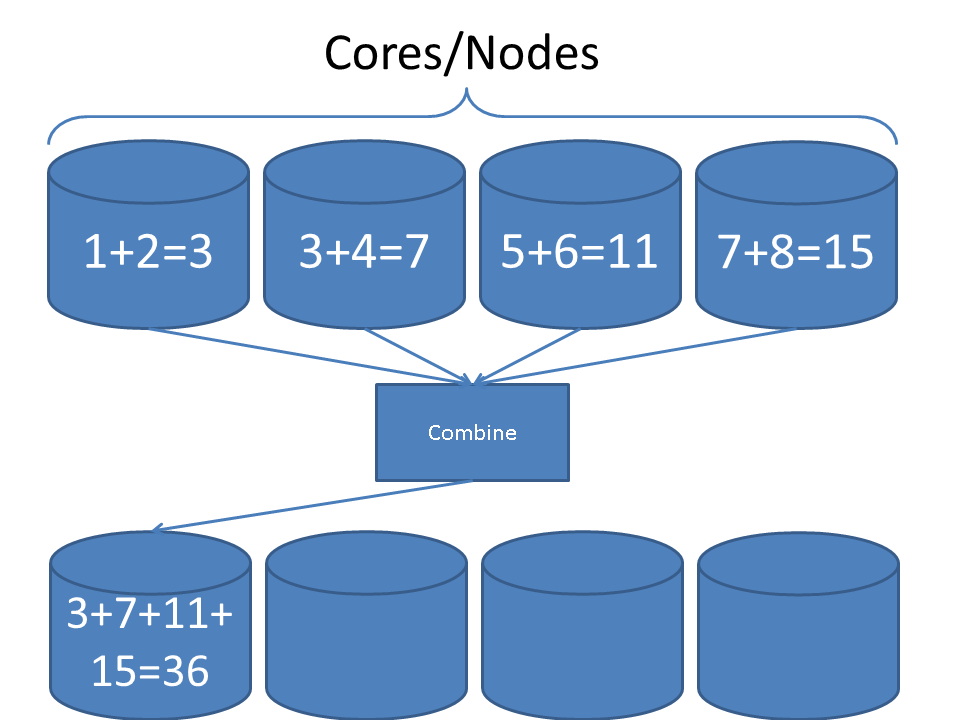
\includegraphics[scale=.45]{pbdDEMO-include/pics/parallelism_data}
 \caption{Task Parallelism Example}
 \label{fig:dataparallel}
\end{figure}
offers a visualization of a very simple data parallelism problem. Say we
have an array consisting of the values 1 through 8, and we have 4 cores
(processing units) at our disposal, and we want to add up all of the elements
of this array. We might distribute the data as in the diagram (the first
two elements of the array on the first core, the next two elements on the
second core, and so on). We then perform a local summation operation;
this local operation is serial, but because we have divided up the overall
task of summation across the multiple processors, for a very large array
we would expect to see performance gains.

A very loose pseudo code for this procedure might look like:

\pseudocode{
  \State $mydata =$ map$(data)$\label{pseudo1:load}
  \State $total\_local =$ sum$(mydata)$
  \State $total = $ reduce$(total\_local)$\label{pseudo1:reduce}
  \If {$this\_processor == processor\_1$}
      \State print$(total)$
  \EndIf
}

Then each of the four cores could execute this code simultaneously, with some
cooperation between the processors for step \ref{pseudo1:load} (in determining
who owns what) and for the reduction in step \ref{pseudo1:reduce}. This is
an example of using a higher-level parallel programming paradigm called
``Single Program/Multiple Data''\index{Single Program/Multiple Data|see{SPMD}}
or SPMD.~\index{Parallelism!SPMD}
We will elucidate more as to exactly what this means in the sections to follow.



\subsubsection{Task Parallelism}

Data parallelism is one parallel programming model. By contrast, another
important parallel programming model is
\emph{task parallelism},\index{Parallelism!task parallelism}
which much of the \proglang{R} community is already fairly adept at. Task
parallelism involves, as the name implies, distributing different execution
tasks across processors. Task parallelism is often
\emph{embarrassingly parallel}\index{Parallelism!embarrassingly parallel} ---
meaning the parallelism is so easy to exploit that it is embarrassing. This
kind of situation occurs when you have complete independence, or a
\emph{loosely coupled} problem (as opposed to something \emph{tightly coupled},
like computing the Singular Value Decomposition
(SVD)~\index{Singular Value Decomposition}\index{Decomposition!SVD} of a
distributed data matrix, for example).  

As a simple example of task parallelism, say you have one dataset and four
processing cores, and you want to fit all four different linear regression
models for that dataset, and then choose the model with lowest
AIC~\citep{aic} (we are not arguing that this is necessarily a good idea; this
is just an example). Fitting one model does not have any dependence on
fitting another, so you might want to just do the obvious thing and have each
core fit a separate model, compute the AIC value locally, then compare all
computed AIC values, lowest is the winner. Figure~\ref{fig:taskparallel} 
\begin{figure}[h]
 \centering
 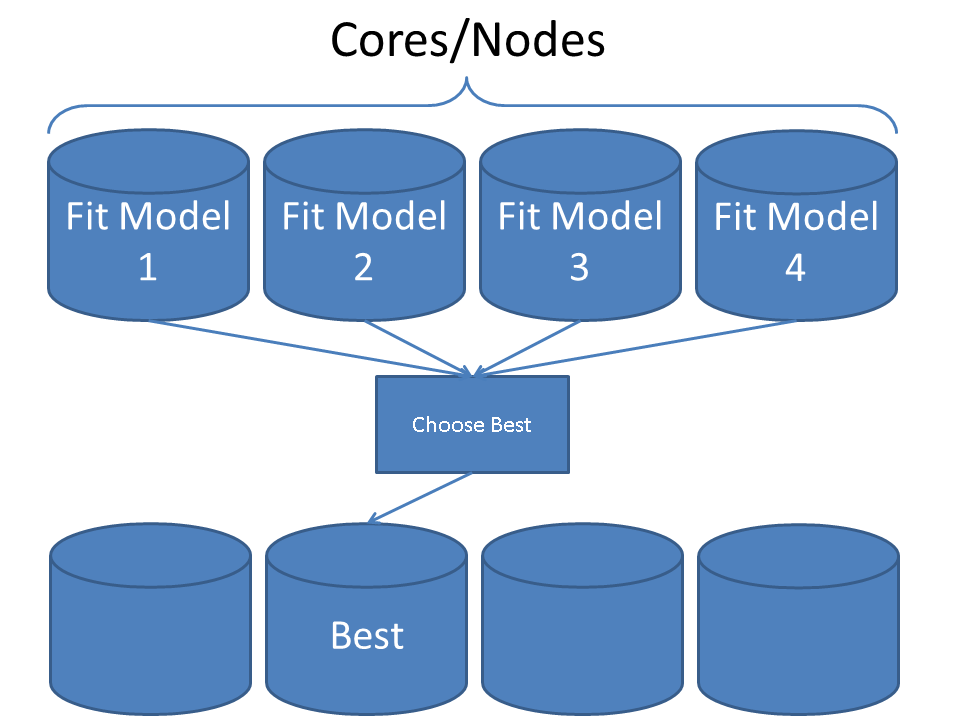
\includegraphics[scale=.45]{pbdDEMO-include/pics/parallelism_task}
 \caption{Task Parallelism Example}
 \label{fig:taskparallel}
\end{figure}
offers a simple visualization of this procedure.


A very loose pseudo code for this problem might look like:

\pseudocode{
  \State load\_data()
  
  \If {$this\_processor == processor\_1$} \label{pseudo2:load}
      \State distribute\_tasks()
  \Else
      \State receive\_tasks()
  \EndIf
  \State $model\_aic =$ aic$($fit$(mymodel))$
  \State $best\_aic = $ min$($allgather$(model\_aic))$\label{pseudo2:gather}
  
  \If {$model\_aic == best\_aic$}
      \State print$(mymodel)$
  \EndIf
}

Then each of the four cores could execute this code simultaneously, with some
cooperation between the processors for the distribution of tasks (which model
to fit) in step \ref{pseudo2:load} and for the gather operation in
step \ref{pseudo2:gather}.


The line between data parallelism and task parallelism sometimes blurs,
especially in simple examples such as those presented here; given our loose
definitions of terms, is our first example really data parallelism?  Or is
it task parallelism?  It is best not to spend too much time worrying about
what to call it and instead focus on how to do it. These are simple examples
and should not be taken too far out of context. All that said, the proverbial
rabbit hole of parallel programming goes quite deep, and often it is not a
matter of one programming model or another, but leveraging several at once
to solve a complicated problem.





\section{SPMD Programming with R}

Throughout this document, we will be using the `Single Program/Multiple Data'',
or SPMD,\index{Parallelism!SPMD} paradigm for distributed computing.
Writing programs in the SPMD style is a very natural way of doing
computations in parallel, but can be somewhat difficult to properly describe.
As the name implies, only one program is written, but the different processors
involved in the computation all execute the code independently on different
portions of the data. The process is arguably the most natural extension of
running serial codes in batch. This model lends itself especially well to
data parallelism problems.

Unfortunately, executing jobs in batch is a somewhat unknown way of doing
business to the typical \proglang{R} user. While details and examples about
this process will be provided in the chapters to follow, the reader is
encouraged to read the \pkg{pbdMPI} package's
vignette~\citep{Chen2012pbdMPIvignette} first.  Ideally, readers should
run the demos of the \pkg{pbdMPI} package, going through the code step by step.




\section{Notation}
\label{sec:notation}

Note that we tend to use suffix
\code{.spmd}\index{Class!\code{.spmd}} for an object when we wish to indicate
that the object is distributed.  This is purely for pedagogical convenience,
and has no semantic meaning. Since the code is written in SPMD style, you
can think of such objects as referring to either a large, global object, or
to a processor's local piece of the whole (depending on context).
This is less confusing than it might first sound.

We will not use this suffix to denote a global object common to all processors.
As a simple example, you could imagine having a large matrix with (global)
dimensions $m\times n$ with each processor owning different collections of
rows of the matrix. All processors might need to know the values for
$m$ and $n$; however, $m$ and $n$ do not depend on the local process, and
so these do not receive the \code{.spmd} suffix. In many cases, it may be
a good idea to invent an S4 class object and a corresponding set of methods.
Doing so can greatly improve the usability and readability of your code, but
is never strictly necessary. However, these constructions are the foundation
of the
\pkg{pbdBASE}~\citep{Schmidt2012pbdBASEpackage} and
\pkg{pbdDMAT}~\citep{Schmidt2012pbdDMATpackage} packages.

On that note, depending on your requirements in distributed computing
with \proglang{R}, it may be beneficial to you to use higher
\proglang{pbdR} toolchain.  If you need to perform dense matrix operations,
or statistical analysis which depend heavily on matrix algebra (linear
modeling, principal components analysis, \dots), then the \pkg{pbdBASE}
and \pkg{pbdDMAT} packages are a natural choice. The major hurdle to using
these tools is getting the data into the appropriate
\code{ddmatrix} format,~\index{Code!\code{ddmatrix}} although we provide
many tools to ease the pains of doing so. Learning how to use these packages
can greatly improve code performance, and take your statistical modeling
in \proglang{R} to previously unimaginable scales.

Again for the sake of understanding, we will at times append the suffix
\code{.dmat}~\index{Class!\code{.dmat}} to objects of class
\code{ddmatrix}\index{Class!\code{ddmatrix}} to differentiate them from the
more general \code{.spmd} object.  As with \code{.spmd}, this carries no
semantic meaning, and is merely used to improve the readability of example
code (especially when managing both ``\code{.spmd}'' and \code{ddmatrix}
objects).




\section{Exercises}
\label{sec:background}

\begin{enumerate}[label=\thechapter-\arabic*]
\item
Read the SPMD wiki page at
\url{http://en.wikipedia.org/wiki/SPMD}
and it's related information.

\item
\proglang{R} users are focusing on task parallelism such as
master/workers framework\index{Parallelism!master/workers framework}
including packages
\pkg{snow}~\citep{Tierney2012}\index{Package!\pkg{snow}},
\pkg{parallel}~\citep{parallel}\index{Package!\pkg{parallel}}, and
\pkg{Rmpi}~\citep{Rmpi}\index{Package!\pkg{Rmpi}}, etc.
Try to identify other packages belongs to or related this class.
{\color{blue}Hint:
``CRAN Task View: High-Performance and Parallel Computing with R'' at
\url{http://cran.r-project.org/web/views/HighPerformanceComputing.html}.
}

\item
Identify particular types or assumptions of Statistical problems which is
particularly beneficial by using the master/workers framework.
Also, identify bottlenecks of this framework and suggest solutions
for the problems.

\item
Multi-threading\index{Parallelism!multi-threading}
and forking\index{Parallelism!forking}
are also popular parallelisms in personal laptop.
The function \code{mclapply()}\index{Code!\code{mclapply()}}
in \pkg{parallel} originated
from \pkg{multicore}~\citep{multicore}\index{Package!\pkg{multicore}}
is for shared memory machines by using
\code{fork} mechanism.
Compare this with OpenMP~\citep{OpenMP}\index{Library!OpenMP}.


\end{enumerate}

